\section{Numerical results}

We now present numerical results for realistic setting. Our experiments
are based on data obtained from New York Presbyterian.

\subsection{Setup}

NY Presbyterian hospital has three different sites across Manhattan.
They are named after their address: York Ave, 55th St and West 84th St.
See Figure \ref{fig:site}. The two sites on each side is very close
to each other, it's only 15min walking distance. The one on west side
is a bit further, it's 15min driving distance without traffic.
Based on this, we think 1 hour lead time is enough for patient to
plan for a different facility.

\begin{figure}
\centering
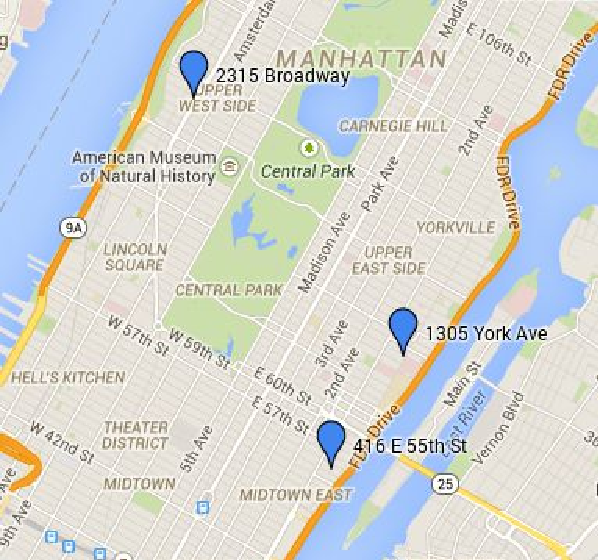
\includegraphics[scale=.6]{chap3/pic/site.pdf}
\caption{Locations of MRI facilities of New York Presbyterian. There
are three in total represented as blue bubbles. Two of them are on
east side and one is on west side.}
\label{fig:site}
\end{figure}

These sites have different number of MRI machines. West 84th has
only one machine. 55th St has two machines. York Ave has four machines.
Since they have different processing capacity, different number of
appointments are scheduled for different facilities. With 4 machines
at York Ave, itself has quite a bit resourcing pooling ability, making
patients there in general wait less.

We have three years data of historical MRI scans. For each of these
scans, we have the type of scan, its appointment time, when patient
arrived, when scan began and when scan finished. From these, we
gathered distribution information about how long it takes for each
type of scans. We use this information in our simulation to make
prediction about future. Another information we use is patients'
arrival time. Based on historical data, we gathered how early/late
patients come respect to their appointment time. We also incorporate
this information in our simulation.

Ideally, we can just replay each day in history and use actual arrival
times and actual scan durations for simulation. However, this is
hard to do. In reality, there are all kinds of issues like cancellation,
same day add-on patients, patients experiencing claustrophobia and cannot
finish their scans, etc. Some issues are not recorded in data, resulting
in weird looking schedule. Some useful critical field is also not tracked
in data and we cannot find a way to reconstruct what appointments are scheduled
in history. To prevent these data issues to corrupt our experiment results,
we decide to conduct our experiment in more controlled way.

We will generate daily schedules similar to what they have everyday. Then,
we will generate the actual scan durations according to distributions we
generated. We will also generate patients arrival time using distribution we
obtained from data. In addition, we also incorporate features like cancellation
and same day add-on patients, where we can randomly generate who will cancel
and when will they cancel, for SDAOP, we can generate when will they come.
Of course, when making decision, we don't assume we know the actual scan durations
and arrival time, it also has no knowledge about SDAOP who haven't shown up.
It also doesn't know who will cancel. When making diversion decision, it can
only use distribution information about these patients.

\subsection{Experiment design}

We want to explore our approach with different scenarios. There are two things
determining how much control our approach can exert on existing schedule.
The first is percentage of volunteer among all patients. With higher percentage
of volunteer, we have more options in term of how can we try to divert.
The other one is lead time, with very long lead time, we won't be able to
make accurate prediction into future. However, longer lead time makes it
more practical for patients.

Thus, in our experiment, we will varying the percentage of patients and
lead time and see their impact on the system performance.

\subsection{Results}

There are several metrics that we look at for system performance.
Figure \ref{fig:60min,fig:90min} shows how
our approach impacts the fraction of patients experiencing extreme long
waiting time. Without interference, there is about 13\% patients waiting
more than 60min and 4\% patients waiting more than 90min. When we
have 40\% patients as volunteers and 60min lead time, only 9.5\% patients
waits more than 60min and 1.2\% patients wait more than 90min.
We can see that with more volunteers, the performance becomes better.
However, cases of extreme waiting time decrease faster when we have
small fraction of volunteers. The reason is that if we have too many
options for volunteers, we won't have that many diversion opportunties.
Another thing is that the difference between 60min and 90min lead time
isn't very big. This is good because it implies with more practical
lead time, our approach can still have a big impact.

\begin{figure}
\centering
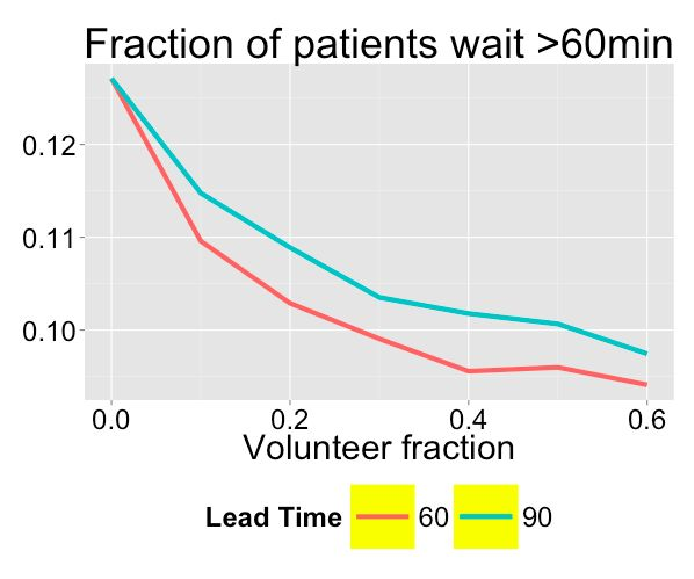
\includegraphics[width=.9\textwidth]{chap3/pic/60min_wait.pdf}
\caption{Fraction of patients wait more than 60min.}
\label{fig:60min}
\end{figure}

\begin{figure}
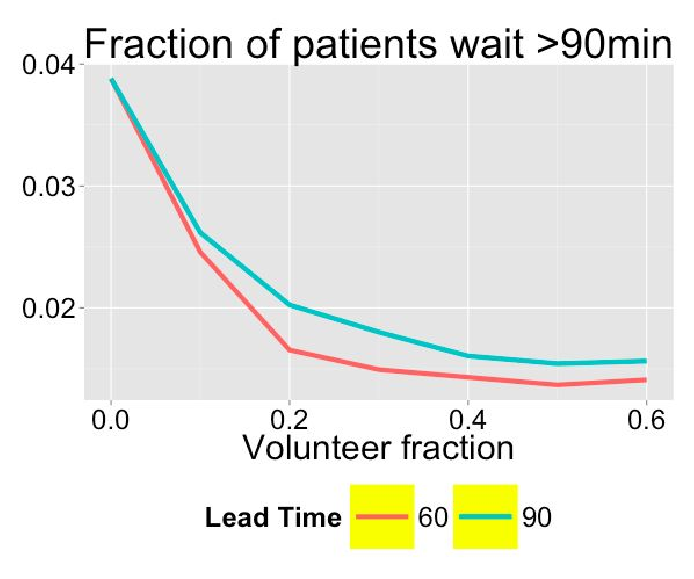
\includegraphics[width=.9\textwidth]{chap3/pic/90min_wait.pdf}
\caption{Fraction of patients wait more than 90min.}
\label{fig:90min}
\end{figure}


Because we divert patients from more congested facility to other
facility, it may cause patients in diverted facility wait more.
But overall, are we gaining or losing on waiting time? Figure
\ref{fig:mean_waiting} is looking into this. As we can see,
we have mild gain in waiting time. We reduce mean waiting time
from 27min to 25.3min with 40\% volunteers and 60min lead time.
This shows that we are not reducing long waiting time cases
totally by propping up short waiting time cases. Although
gain of 1.7min on mean waiting time doesn't seem much, but
this is average over all patients and lots of them are not
impacted by our diversions. To explain the reason why
we can gain on mean waiting time, we refer to the fact that
our diversion will actual reduce idle time of machines. This
comes in two reaons: the first is that we may divert patients
to some time slot that's not utilized, the second is that
by balancing demand, it's less likely idle time developed because
some scan takes less than expected time.

\begin{figure}
\centering
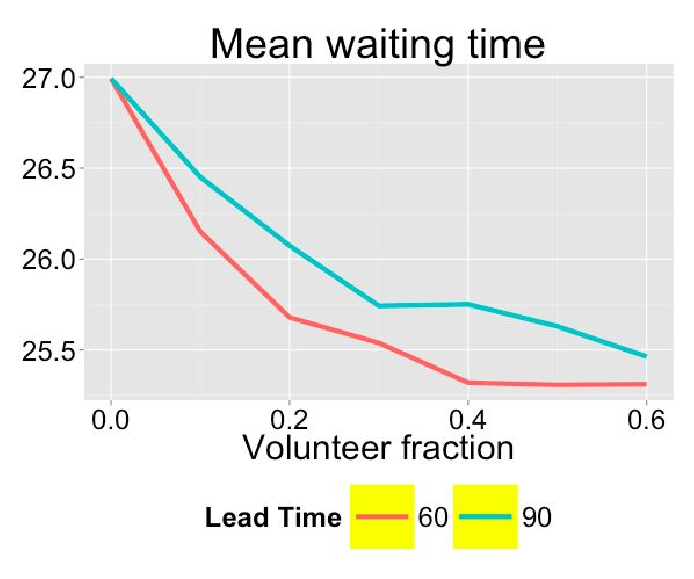
\includegraphics[width=.9\textwidth]{chap3/pic/mean_waiting.pdf}
\caption{Mean waiting time.}
\label{fig:mean_waiting}
\end{figure}

The last thing we look at is how much trouble do we incur to
implement this diversion policy. Figure \ref{fig:fraction}
shows how much patients we actually end up diverting. Even with
60\% patients, we at most divert 2.5\% patients. This means
in daily operation, we on average only need to divert a handful
of people throughout the whole day. The low cost of implementing
diversion policy, together with the benefits it can bring, justifies
the implementation of this policy.

\begin{figure}
\centering
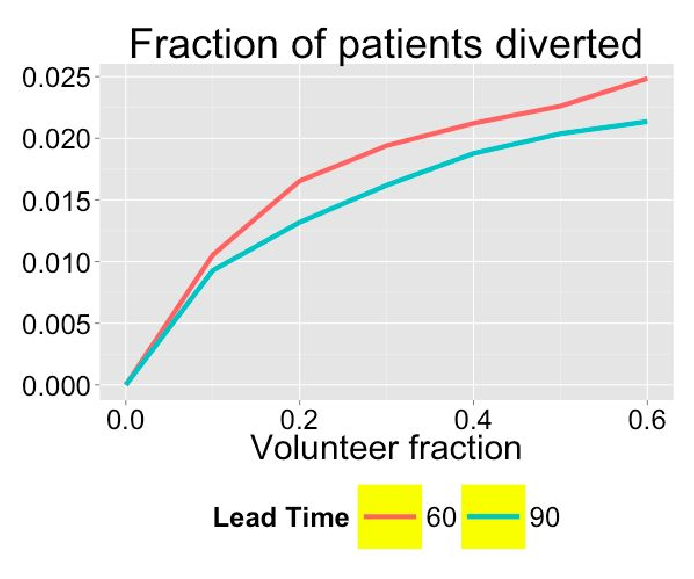
\includegraphics[width=.9\textwidth]{chap3/pic/fraction.pdf}
\caption{Fraction of diverted patients.}
\label{fig:fraction}
\end{figure}
